\documentclass[letterpaper,10pt]{article}

\usepackage{enumitem}
\usepackage{titling}
\usepackage{listings,listings-rust}
\usepackage{url}
\usepackage{soul}
\usepackage{hyperref}
\usepackage{setspace}
\usepackage{subfig}
\usepackage{sectsty}
\usepackage{pdfpages}
\usepackage{colortbl}
\usepackage{multirow}
\usepackage{multicol}
\usepackage{relsize}
\usepackage{amsmath}
\usepackage{wasysym}
\usepackage{fancyvrb}
\usepackage[yyyymmdd]{datetime}
\usepackage{amsmath,amssymb,amsthm,graphicx,xspace}
\usepackage[titlenotnumbered,noend,noline]{algorithm2e}
\usepackage[compact]{titlesec}
\usepackage{XCharter}
\usepackage[T1]{fontenc}
\usepackage[scaled]{beramono}
\usepackage[normalem]{ulem}
\usepackage{booktabs}
\usepackage{tikz}
\usetikzlibrary{arrows.meta,automata,shapes,trees,matrix,chains,scopes,positioning,calc,decorations.pathreplacing}
\tikzstyle{block} = [rectangle, draw, fill=blue!20, 
    text width=2.5em, text centered, rounded corners, minimum height=2em]
\tikzstyle{bw} = [rectangle, draw, fill=blue!20, 
    text width=4em, text centered, rounded corners, minimum height=2em]

\definecolor{namerow}{cmyk}{.40,.40,.40,.40}
\definecolor{namecol}{cmyk}{.40,.40,.40,.40}
\renewcommand{\dateseparator}{-}

\let\LaTeXtitle\title
\renewcommand{\title}[1]{\LaTeXtitle{\textsf{#1}}}

\lstset{basicstyle=\footnotesize\ttfamily,breaklines=true}

\newcommand{\CPP}{C\nolinebreak\hspace{-.05em}\raisebox{.4ex}{\tiny\bf +}\nolinebreak\hspace{-.10em}\raisebox{.4ex}{\tiny\bf +}}
\def\CPP{{C\nolinebreak[4]\hspace{-.05em}\raisebox{.4ex}{\tiny\bf ++}}}

\newcommand{\handout}[5]{
  \noindent
  \begin{center}
  \framebox{
    \vbox{
      \hbox to 5.78in { {\bf ECE459: Programming for Performance } \hfill #2 }
      \vspace{4mm}
      \hbox to 5.78in { {\Large \hfill #4  \hfill} }
      \vspace{2mm}
      \hbox to 5.78in { {\em #3 \hfill \today} }
    }
  }
  \end{center}
  \vspace*{4mm}
}

\newcommand{\lecture}[3]{\handout{#1}{#2}{#3}{Lecture#1}}
\newcommand{\tuple}[1]{\ensuremath{\left\langle #1 \right\rangle}\xspace}

\addtolength{\oddsidemargin}{-1.000in}
\addtolength{\evensidemargin}{-0.500in}
\addtolength{\textwidth}{2.0in}
\addtolength{\topmargin}{-1.000in}
\addtolength{\textheight}{1.75in}
\addtolength{\parskip}{\baselineskip}
\setlength{\parindent}{0in}
\renewcommand{\baselinestretch}{1.5}
\newcommand{\term}{Winter 2020}

\singlespace


\begin{document}

\lecture{28 --- Profiler Guided Optimization (POGO)}{\term}{Jeff Zarnett}

\section*{Profiler Guided Optimization (POGO)}

In 2015 we were fortunate enough to have a guest lecture from someone at Microsoft actually in the room to give the guest lecture on the subject of Profile Guided Optimization (or POGO). Try as I might, I was not able to convince him to fly in just for this lecture. For an alternative take on the subject, you could watch the full video at \url{https://www.youtube.com/watch?v=zEsdBcu4R00}. We'll use an excerpt in this lecture.

The compiler does a great deal of static analysis of the code you've written and makes its best guesses about what is likely to happen. The canonical example for this is branch prediction: there is an if-else block and the compiler will then guess about which is more likely and optimize for that version. Consider three examples from~\cite{pogo}:

\begin{center}
	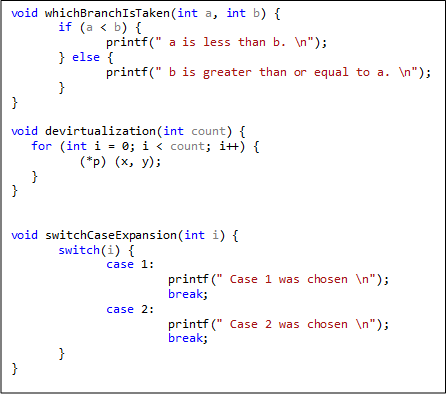
\includegraphics[width=0.5\textwidth]{images/4621codesnippet.png}
\end{center}

Just looking at this, which is more likely, \texttt{a > b} or \texttt{a <= b}? Assuming there's no other information in the system the compiler can believe that one is more likely than the other, or having no real information, use a fallback rule. This works, but what if we are wrong? Suppose the compiler decides it is likely that \texttt{a} is the larger value and it optimizes for that version. However, it is only the case 5\% of the time, so most of the time the prediction is wrong. That's unpleasant. But the only way to know is to actually run the program.

There are similar questions raised for the other two examples. What is the ``normal'' value for some pointer \texttt{p}? If we do not know, the compiler cannot do devirtualization (replace this virtual call with a real one). Same thing with \texttt{i}: what is its typical value? If we know that, it is our prediction. Actually, in a switch-case block with many options, could we rank them in descending order of likelihood?

There exists a solution to this, and it is that we can give hints to the compiler, but that's a manual process. Automation is a good thing and this lecture is about that. These sorts of things already exist for Java! The Java HotSpot virtual machine will update its predictions on the fly. There are some initial predictions and if they turn out to be wrong, the Just In Time compiler will replace it with the other version. That's neat! I don't know for certain but I suspect the .NET runtime will do the same for something like C\#. But this is C(++) (Sparta) and we don't have that: the compiler runs and it does its job and that's it; the program is never updated with newer predictions if more data becomes known.

Solving this problem is the goal of POGO. It is taking the data from some actual runs of the program and using that to inform the predictions. This necessitates a multi-step compile: first compile the code, run it to collect data, then recompile the code using the data we collected. Let's expand on all three steps.

Step one is to generate an executable with instrumentation. The compiler inserts a bunch of probes into the generated code that are used to record data. Three types of probe are inserted: function entry probes, edge probes, and value probes.  A function entry probe, obviously, counts how many times a particular function is called. An edge probe is used to count the transitions (which tells us whether an if branch is taken or the else condition). Value probes are interesting; they are used to collect a histogram of values. Thus, we can have a small table that tells us the frequency of what is given in to a \texttt{switch} statement. When this phase is complete, there is an instrumented executable and an empty database file where the training data goes~\cite{pogo}.

Step two is training day: run the instrumented executable through real-world scenarios. Ideally you will spend the training time on the performance-critical sections. It does not have to be a single training run, of course, data can be collected from as many runs as desired.   Still, it is important to note that you are not trying to exercise every part of the program (this is not unit testing); instead it should be as close to real-world-usage as can be accomplished. In fact, trying to use ever bell and whistle of the program is counterproductive; if the usage data does not match real world scenarios then  the compiler has been given the wrong information about what is important. Or you might end up teaching it that almost nothing is important...

Step three is a recompile. This time, in addition to the source files, the training data is fed into the compiler for a second compile. and this data is applied to produce a better output executable than could be achieved by static analysis alone.

The Intel Developer Zone explains the process in a handy infographic\footnote{Source: \url{https://software.intel.com/en-us/node/522721}} :

\begin{center}
	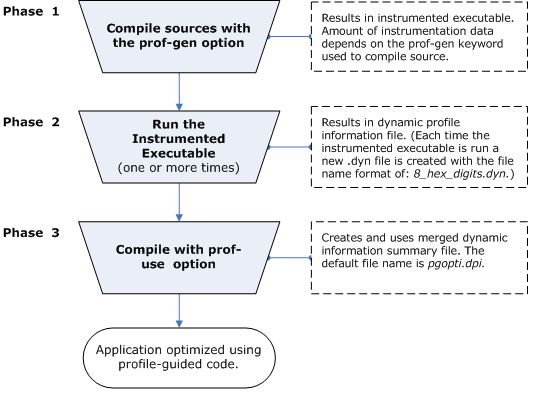
\includegraphics[width=0.5\textwidth]{images/pogo-workflow.jpg}
\end{center}

It is not necessary to do all three steps for every build. Old training data can be re-used until the code base has diverged significantly enough from the instrumented version. According to~\cite{pogo}, the recommended workflow is for one developer to perform these steps and check the training data into source control so that other developers can make use of it in their builds.

What does it mean for it to be better? We have already looked at an example about how to predict branches. Predicting it correctly will be faster than predicting it incorrectly, but this is not the only thing.  The algorithms will aim for speed in the areas that are ``hot'' (performance critical and/or common scenarios). The algorithms will alternatively aim to minimize the size of code of areas that are ``cold'' (not heavily used). It is recommended in~\cite{pogo} that less than 5\% of methods should be compiled for speed.

It is possible that we can combine multiple training runs and we can manually give some suggestions of what scenarios are important. Obviously the more a scenario runs in the training data, the more important it will be, as far as the POGO optimization routine is concerned, but multiple runs can be merged with user assigned weightings.

With the theory behind us, perhaps a demonstration about how it works is in order. Let us consider an example using the N-Body problem. Let's look at the video \url{https://www.youtube.com/watch?v=zEsdBcu4R00&t=21m45s} (from 21:45 to 34:23). (We'll come back to the video again in a little bit to see more of it at the end.)


\subsection*{Behind the Scenes}

In the optimize phase, the training data is used to do the following optimizations~\cite{pogo2}:

\begin{multicols}{2}
\begin{enumerate}
\item Full and partial inlining
\item Function layout
\item Speed and size decision
\item Basic block layout 
\item Code separation
\item Virtual call speculation
\item Switch expansion
\item Data separation
\item Loop unrolling
\end{enumerate}
\end{multicols}

For the most part we should be familiar with the techniques that are listed as being other compiler optimizations we have previously discussed. The new ones are (3) speed and size decision, which we have just covered; and items (4) and (5) which relate to how to pack the generated code in the binary.

According to~\cite{pogo2} the majority of the performance gains relate to the inlining decisions. These decisions are based on the call graph path profiling: the behaviour of function \texttt{foo} may be very different when calling it from \texttt{bar} than it is when calling it from function \texttt{baz}\footnote{Why are these the example function names?! It's kind of like Alice and Bob...}. Great, let's look at this call graph from~\cite{pogo2}:

\begin{center}
	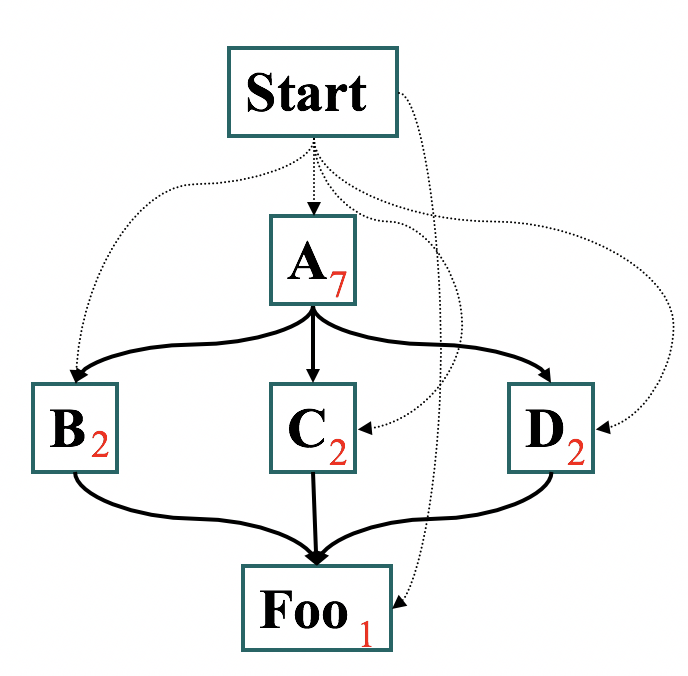
\includegraphics[width=0.25\textwidth]{images/callpaths.png}
\end{center}

Quick analysis of this code would have us find all the ways in which the functions might call each other. In total, there are 14 paths in this code, seven of which get us to function \texttt{Foo}.  

Consider another diagram showing the relationships between functions, in which the numbers on the edges represent the number of invocations~\cite{pogo2}:

\begin{center}
	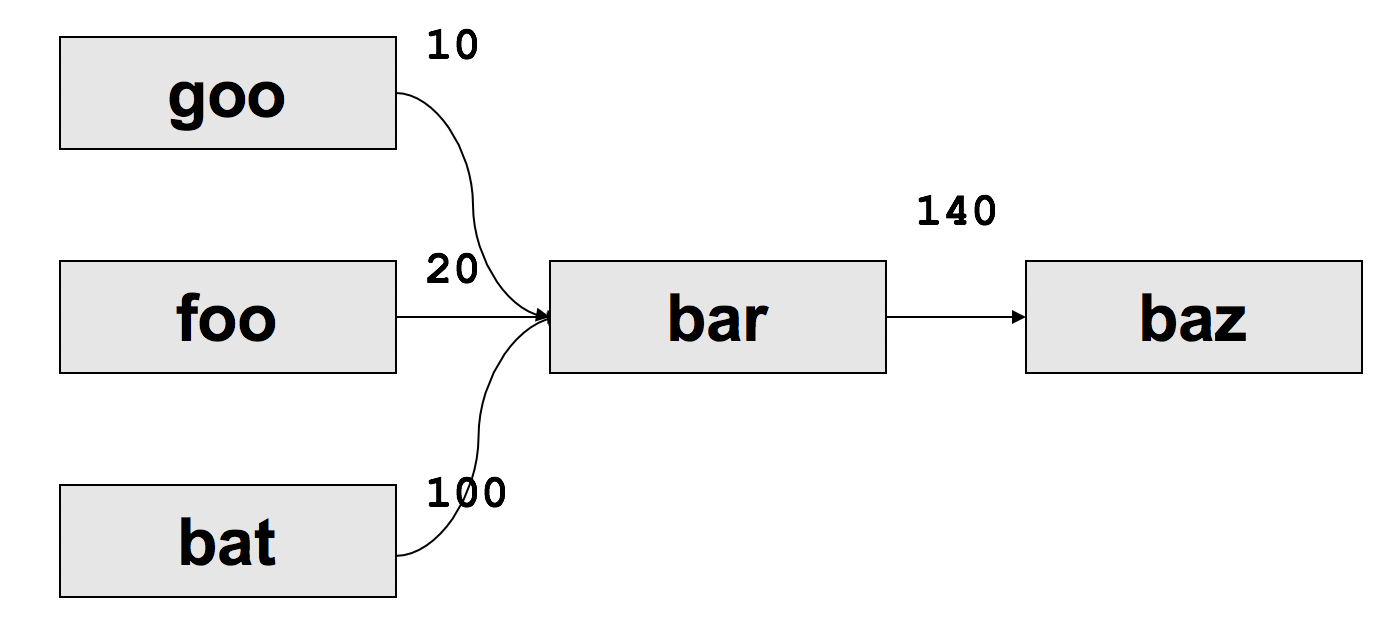
\includegraphics[width=0.4\textwidth]{images/callpaths2.png}
\end{center}

When considering what to do here, POGO takes the view like this~\cite{pogo2}:

\begin{center}
	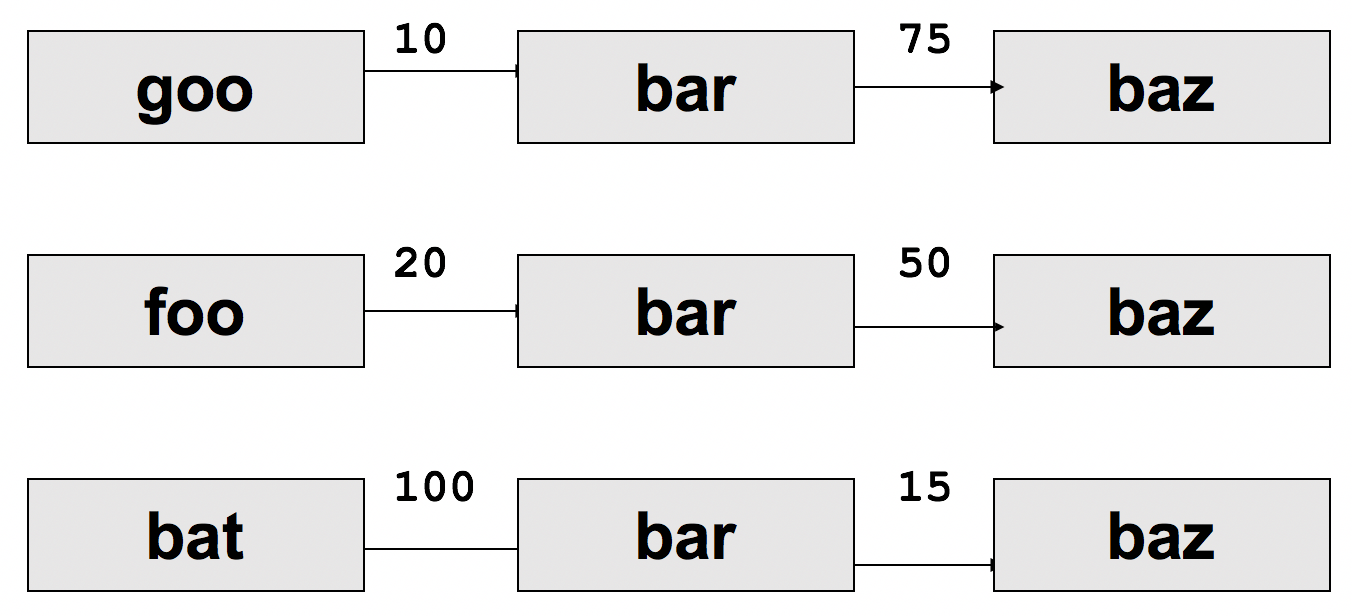
\includegraphics[width=0.4\textwidth]{images/callpaths3.png}
\end{center}

Each part of the call path is considered separately, remembering that we want to inline where it makes sense for speed, but otherwise leave it alone because of code size increases. Inlining \texttt{bar} into \texttt{bat} makes sense, but not inlining \texttt{bar} into \texttt{goo} (because that increases the code size without significant performance benefits). It also makes sense for \texttt{baz} to get inlined into \texttt{bar}. This is illustrated below~\cite{pogo2}:

\begin{center}
	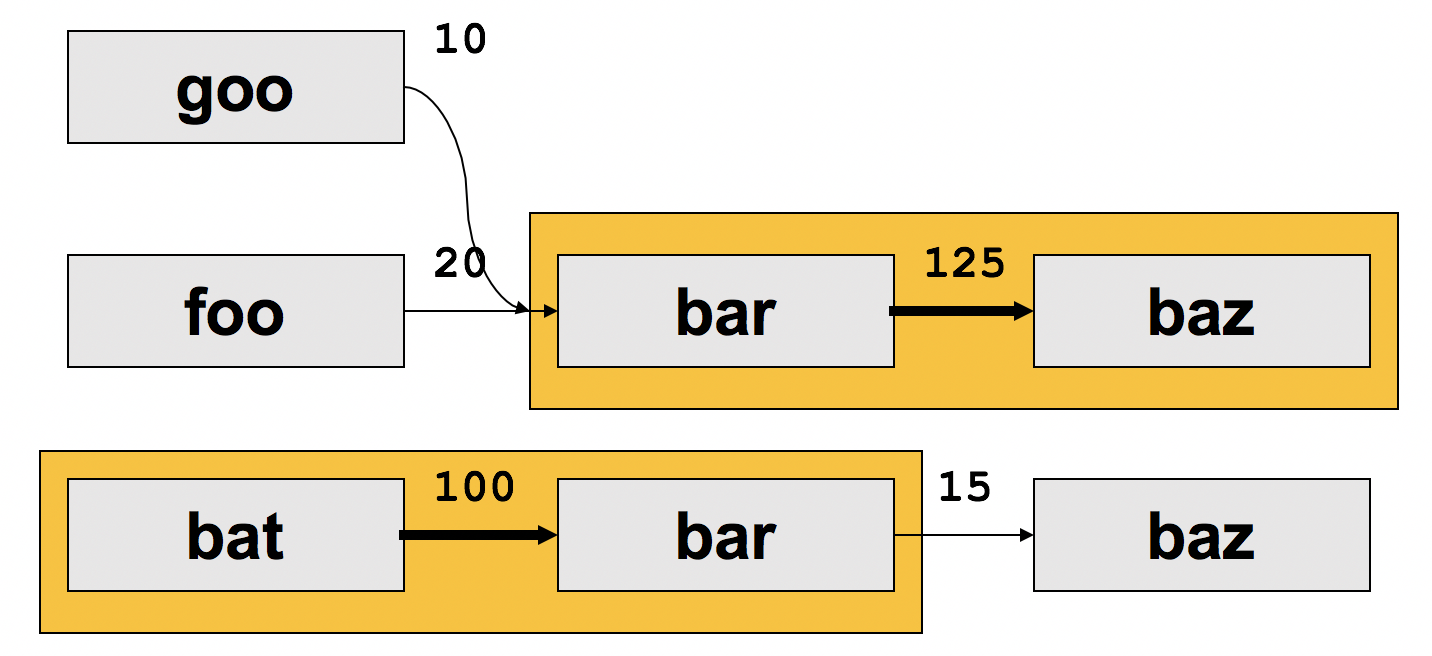
\includegraphics[width=0.4\textwidth]{images/callpaths4.png}
\end{center}

Packing the blocks is also done based on this call graph profiling. The most common cases will be put next to each other, and, where possible, subsequent steps are put next to each other. The more we can pack related code together, the fewer page faults we get by jumping to some other section, causing a cache miss... If the function being called is in the same page as the call, it has achieved ``page locality'' (and that is the goal!). This is represented visually~\cite{pogo2}:

\begin{center}
	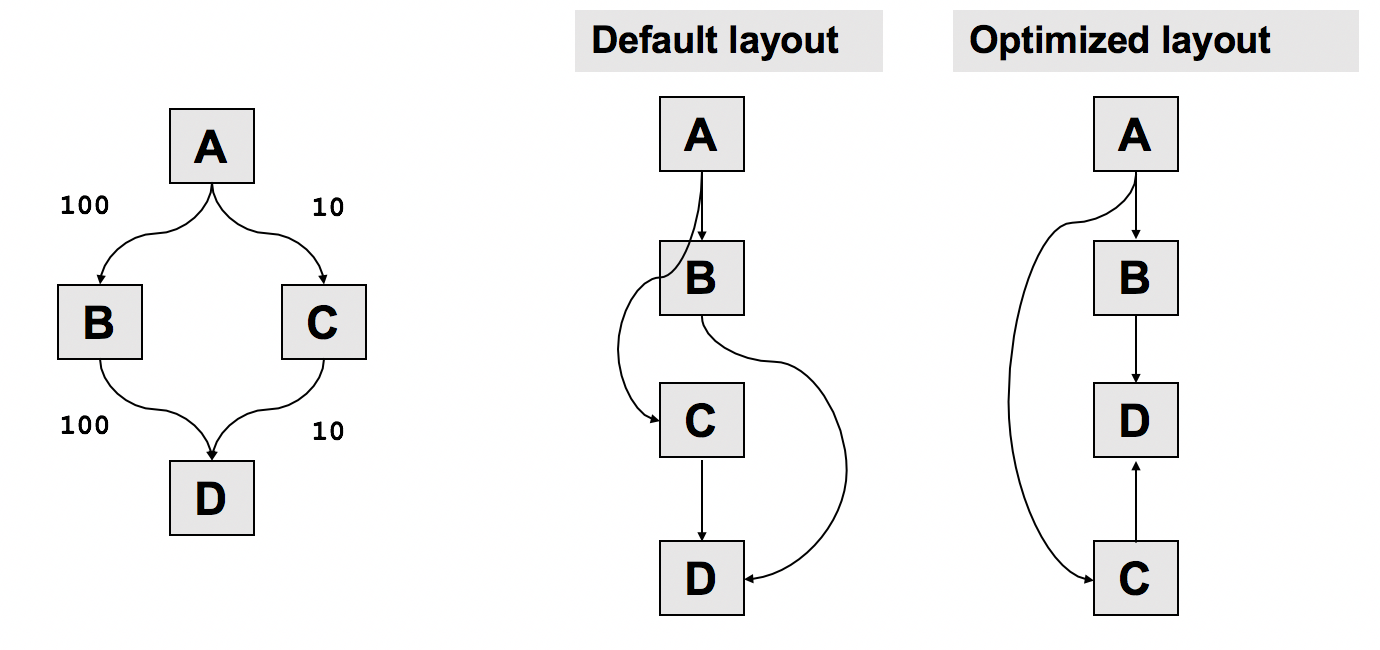
\includegraphics[width=0.6\textwidth]{images/blocklayout.png}
\end{center}

According to the author, the ``dead'' code goes in its own special block. I don't think they actually mean truly dead code, the kind that is compile-time determined to be unreachable, but instead they mean code that never gets invoked in any of the training runs.

So, to sum up, the training data is used to identify what branches are likely to be taken, inlines code where that is a performance increase, and tries to pack the binary code in such a way as to reduce cache misses/page faults. How well does it work?

\subsection*{Benchmark Results}

This table, condensed from~\cite{pogo2} summarizes the gains to be made. The application under test is a standard benchmark suite (Spec2K):

\begin{center}
\begin{tabular}{l|l|l|l|l|l}
	\textbf{Spec2k:} & \textbf{sjeng} & \textbf{gobmk} & \textbf{perl} & \textbf{povray} & \textbf{gcc}\\ \hline
	\textbf{App Size:} &  {Small} & {Medium} & {Medium} & {Medium} & {Large} \\ \hline
	\textbf{Inlined Edge Count} & 50\% & 53\% & 25\% & 79\% & 65\% \\ \hline
	\textbf{Page Locality} & 97\% & 75\% & 85\% & 98\% & 80\% \\ \hline
	\textbf{Speed Gain} & 8.5\% & 6.6\% & 14.9\% & 36.9\% & 7.9\% \\ 
\end{tabular}
\end{center}

There are more details in the source as to how many functions are used in a typical run and how many things were inlined and so on. But we get enough of an idea from the last row of how much we are speeding up the program, plus some information about why. We can speculate about how well the results in a synthetic benchmark translate to real-world application performance, but at least from this view it does seem to be a net gain.

\bibliographystyle{alphaurl}
\bibliography{459}

\end{document}
